
\chapter{THỬ NGHIỆM VÀ KẾT QUẢ}

% ============================================
% 4.1. THIẾT LẬP THỰC NGHIỆM
% ============================================

\section{Môi trường và thiết lập thực nghiệm}

\subsection{Môi trường thực nghiệm}

Các thí nghiệm của đề tài được thực hiện bằng ngôn ngữ
Python trên môi trường Jupyter Notebook thông qua Visual
Studio Code.

Nhóm sử dụng các thư viện Pandas, NumPy, SciPy và
Scikit-learn để xử lý dữ liệu, biểu diễn đặc trưng, huấn
luyện và đánh giá mô hình. Matplotlib và Seaborn được
sử dụng để trực quan hóa các kết quả thực nghiệm.

Những thí nghiệm được triển khai trong các notebook
\texttt{02\_Preprocessing.ipynb},
\texttt{03\_Training.ipynb} và
\texttt{04\_Evaluation.ipynb}.

Các kết quả được trình bày trong chương này được tổng
hợp từ dữ liệu và đầu ra thực tế của chương trình.

\subsection{Dữ liệu thực nghiệm}

Nhóm sử dụng bộ dữ liệu phản hồi sinh viên đã được
khám phá và phân tích trong Chương 1.

Sau các bước kiểm tra chất lượng và làm sạch dữ liệu,
số lượng phản hồi được giữ lại là 1.223 mẫu, thuộc
ba lớp cảm xúc: negative, neutral và positive.

Dữ liệu được chia thành hai tập theo tỷ lệ 80/20,
sử dụng \texttt{random\_state=42} và phân tầng
theo nhãn mục tiêu.

Kết quả phân chia được trình bày trong
Bảng~\ref{tab:ch4-chia-du-lieu}.

\begin{table}[H]
\centering
\caption{Phân chia dữ liệu thực nghiệm}
\label{tab:ch4-chia-du-lieu}
\renewcommand{\arraystretch}{1.15}

\begin{tabular}{|l|r|r|r|}
\hline
\textbf{Nhãn}
& \textbf{Train}
& \textbf{Test}
& \textbf{Tổng} \\
\hline
Negative & 293 & 73 & 366 \\
\hline
Neutral & 294 & 74 & 368 \\
\hline
Positive & 391 & 98 & 489 \\
\hline
\textbf{Tổng}
& \textbf{978}
& \textbf{245}
& \textbf{1.223} \\
\hline
\end{tabular}
\end{table}

Tập train gồm 978 phản hồi, được sử dụng để xây dựng
bộ đặc trưng, huấn luyện và lựa chọn siêu tham số.

Tập test gồm 245 phản hồi, được giữ riêng để đánh
giá các cấu hình sau khi hoàn tất quá trình lựa chọn
tham số trên tập train.

Nhóm không sử dụng tập test trong quá trình
GridSearchCV nhằm hạn chế hiện tượng rò rỉ dữ liệu.

\subsection{Các phương án thực nghiệm}

Nhóm tiến hành thử nghiệm hai thuật toán phân loại
là Multinomial Naive Bayes và K-Nearest Neighbors
(K-NN).

Mỗi thuật toán được kết hợp với bốn phương pháp
biểu diễn văn bản:

\begin{itemize}
    \item Bag-of-Words với unigram.
    \item Bag-of-Words với unigram và bigram.
    \item TF-IDF với unigram.
    \item TF-IDF với unigram và bigram.
\end{itemize}

Như vậy, nhóm xây dựng tám tổ hợp biểu diễn
đặc trưng và thuật toán phân loại.

Để thuận tiện cho các bảng kết quả, nhóm sử dụng
những ký hiệu viết tắt sau:

\begin{itemize}
    \item BoW-U: Bag-of-Words Unigram.
    \item BoW-UB: Bag-of-Words Unigram và Bigram.
    \item TF-U: TF-IDF Unigram.
    \item TF-UB: TF-IDF Unigram và Bigram.
    \item NB: Multinomial Naive Bayes.
    \item KNN: K-Nearest Neighbors.
\end{itemize}

Bên cạnh tám tổ hợp chính, nhóm sử dụng một
baseline BoW-U kết hợp Naive Bayes với
$\alpha=1,0$ và một DummyClassifier để
làm mốc tham khảo.

Các siêu tham số được lựa chọn bằng Stratified
3-Fold Cross-Validation trên tập train, sử dụng
Macro F1-score làm tiêu chí đánh giá.

% ============================================
% 4.2. KẾT QUẢ BASELINE
% ============================================

\section{Kết quả mô hình baseline}

Để có cơ sở so sánh các phương án thử nghiệm,
nhóm xây dựng mô hình baseline sử dụng
Bag-of-Words Unigram kết hợp Multinomial Naive Bayes
với tham số $\alpha=1,0$.

Đồng thời, DummyClassifier sử dụng chiến lược
\texttt{most\_frequent} được triển khai như
một mốc tham khảo đơn giản.

Kết quả đánh giá hai phương án trên tập test
được trình bày trong Bảng~\ref{tab:ch4-baseline}.

\begin{table}[H]
\centering
\caption{Kết quả đánh giá các mô hình tham chiếu}
\label{tab:ch4-baseline}
\renewcommand{\arraystretch}{1.15}
\small

\begin{tabularx}{\textwidth}{|X|r|r|r|r|}
\hline
\textbf{Mô hình}
& \textbf{Accuracy}
& \textbf{P macro}
& \textbf{R macro}
& \textbf{F1 macro} \\
\hline

DummyClassifier
& 0,4000
& 0,1333
& 0,3333
& 0,1905 \\
\hline

BoW-U + NB (Baseline)
& 0,3878
& 0,3764
& 0,3751
& 0,3748 \\
\hline

\end{tabularx}
\end{table}

Trong đó, P macro và R macro lần lượt biểu thị
Precision và Recall được tính theo Macro-average.

Kết quả cho thấy DummyClassifier đạt Accuracy
40,00\%, nhưng Macro F1-score chỉ đạt 0,1905.

Nguyên nhân trực tiếp của kết quả này là phương
pháp Dummy chỉ dự đoán lớp phổ biến nhất trong tập
train, không sử dụng nội dung phản hồi để phân biệt
các lớp cảm xúc.

Trong khi đó, baseline BoW-U kết hợp Naive Bayes
đạt Accuracy 38,78\% và Macro F1-score 0,3748.

Mặc dù Accuracy của baseline thấp hơn Dummy,
Macro F1-score cao hơn đáng kể. Điều này cho thấy
cần kết hợp nhiều chỉ số đánh giá khi xem xét
hiệu quả của bài toán phân loại ba lớp.

Baseline BoW-U kết hợp Naive Bayes được sử dụng
làm mốc chính trong các phần so sánh tiếp theo.

% ============================================
% 4.3. CROSS-VALIDATION
% ============================================

\section{Kết quả kiểm định chéo và lựa chọn siêu tham số}

\subsection{Kết quả Cross-Validation}

Để lựa chọn tham số, nhóm áp dụng
Stratified 3-Fold Cross-Validation trên tập train.

Đối với Multinomial Naive Bayes, các giá trị
$\alpha$ được thử nghiệm gồm 0,5; 1,0 và 2,0.

Đối với K-NN, số láng giềng $k$ được thử nghiệm
với các giá trị 3, 5 và 7.

Tổng cộng có 24 lượt thử tham số, tương ứng với
tám tổ hợp biểu diễn--thuật toán, mỗi tổ hợp
gồm ba giá trị tham số.

Kết quả tốt nhất theo Macro F1-score của từng
tổ hợp được trình bày trong
Bảng~\ref{tab:ch4-ketqua-cv}.

\begin{table}[H]
\centering
\caption{Kết quả Cross-Validation trên tập train}
\label{tab:ch4-ketqua-cv}
\renewcommand{\arraystretch}{1.15}
\small

\begin{tabularx}{\textwidth}{|X|c|r|}
\hline
\textbf{Cấu hình}
& \textbf{Tham số tốt nhất}
& \textbf{F1 macro CV} \\
\hline

BoW-U + NB
& $\alpha=0,5$
& 0,3637 \\
\hline

BoW-U + KNN
& $k=5$
& 0,3555 \\
\hline

BoW-UB + NB
& $\alpha=0,5$
& 0,3569 \\
\hline

BoW-UB + KNN
& $k=7$
& 0,3433 \\
\hline

TF-U + NB
& $\alpha=0,5$
& 0,3374 \\
\hline

\textbf{TF-U + KNN}
& $\boldsymbol{k=5}$
& \textbf{0,3647} \\
\hline

TF-UB + NB
& $\alpha=0,5$
& 0,2852 \\
\hline

TF-UB + KNN
& $k=3$
& 0,3490 \\
\hline

\end{tabularx}
\end{table}

Kết quả cho thấy cấu hình TF-IDF Unigram kết hợp
K-NN với $k=5$ đạt Macro F1-score trung bình cao
nhất trên Cross-Validation, bằng 0,3647.

Cấu hình đứng thứ hai là BoW Unigram kết hợp
Naive Bayes với $\alpha=0,5$, đạt 0,3637.

Mức chênh lệch giữa hai cấu hình chỉ khoảng 0,0010.

Đây là mức chênh lệch nhỏ, chưa đủ cơ sở để khẳng
định cấu hình đứng đầu có hiệu quả vượt trội ổn định.

Tuy nhiên, theo tiêu chí lựa chọn đã thiết lập
trước đó, nhóm lựa chọn TF-IDF Unigram kết hợp
K-NN với $k=5$ làm mô hình được đánh giá chính.

Việc lựa chọn này được thực hiện hoàn toàn dựa
trên kết quả kiểm định chéo của tập train.

\subsection{Ảnh hưởng của siêu tham số}

Bên cạnh việc lựa chọn cấu hình tốt nhất,
nhóm tiến hành so sánh mức thay đổi của Macro
F1-score khi điều chỉnh $\alpha$ và $k$.

Bảng~\ref{tab:ch4-anh-huong-tham-so} trình bày
giá trị tham số có điểm CV cao nhất, thấp nhất
và mức chênh lệch của từng tổ hợp.

\begin{table}[H]
\centering
\caption{Ảnh hưởng của siêu tham số trên Cross-Validation}
\label{tab:ch4-anh-huong-tham-so}
\renewcommand{\arraystretch}{1.12}
\small

\begin{tabularx}{\textwidth}{|X|c|r|c|r|}
\hline
\textbf{Cấu hình}
& \textbf{Tốt nhất}
& \textbf{F1 CV}
& \textbf{Kém nhất}
& \textbf{F1 CV} \\
\hline

BoW-U + NB
& 0,5 & 0,3637
& 2,0 & 0,3564 \\
\hline

BoW-U + KNN
& 5 & 0,3555
& 7 & 0,3413 \\
\hline

BoW-UB + NB
& 0,5 & 0,3569
& 2,0 & 0,3390 \\
\hline

BoW-UB + KNN
& 7 & 0,3433
& 3 & 0,3374 \\
\hline

TF-U + NB
& 0,5 & 0,3374
& 2,0 & 0,2834 \\
\hline

TF-U + KNN
& 5 & 0,3647
& 3 & 0,3489 \\
\hline

TF-UB + NB
& 0,5 & 0,2852
& 2,0 & 0,2048 \\
\hline

TF-UB + KNN
& 3 & 0,3490
& 7 & 0,3445 \\
\hline

\end{tabularx}
\end{table}

Trong các giá trị tham số được thử nghiệm,
Naive Bayes đạt điểm CV cao nhất với
$\alpha=0,5$ ở cả bốn cấu hình biểu diễn.

Đối với K-NN, giá trị $k$ tốt nhất thay đổi theo
phương pháp biểu diễn văn bản. Cụ thể, các giá trị
được lựa chọn là 5, 7 hoặc 3 tùy cấu hình.

Kết quả cho thấy việc thay đổi siêu tham số có
ảnh hưởng đến chất lượng phân loại. Mức độ ảnh
hưởng không giống nhau giữa các cấu hình.

Tuy nhiên, những nhận xét trên được rút ra trong
phạm vi các giá trị đã thử nghiệm và không khẳng
định đây là những tham số tối ưu cho mọi bộ dữ liệu.

% ============================================
% 4.4. ĐÁNH GIÁ TRÊN TEST
% ============================================

\section{Kết quả đánh giá trên tập kiểm thử}

\subsection{So sánh các phương án phân loại}

Sau khi hoàn thành lựa chọn siêu tham số bằng
Cross-Validation, nhóm đánh giá các cấu hình
trên cùng tập test gồm 245 phản hồi.

Kết quả được trình bày trong
Bảng~\ref{tab:ch4-ketqua-test}.

\begin{table}[H]
\centering
\caption{So sánh các phương án trên tập kiểm thử}
\label{tab:ch4-ketqua-test}
\renewcommand{\arraystretch}{1.12}
\small
\setlength{\tabcolsep}{4pt}

\begin{tabularx}{\textwidth}{|X|r|r|r|r|}
\hline
\textbf{Phương án}
& \textbf{Accuracy}
& \textbf{P macro}
& \textbf{R macro}
& \textbf{F1 macro} \\
\hline

DummyClassifier
& 0,4000 & 0,1333 & 0,3333 & 0,1905 \\
\hline

Baseline BoW-U + NB
& 0,3878 & 0,3764 & 0,3751 & 0,3748 \\
\hline

BoW-U + NB
& 0,3837 & 0,3727 & 0,3706 & 0,3702 \\
\hline

BoW-U + KNN
& 0,3592 & 0,3670 & 0,3618 & 0,3588 \\
\hline

BoW-UB + NB
& 0,3673 & 0,3557 & 0,3481 & 0,3436 \\
\hline

BoW-UB + KNN
& 0,3347 & 0,3270 & 0,3275 & 0,3271 \\
\hline

TF-U + NB
& 0,3918 & 0,3801 & 0,3683 & 0,3614 \\
\hline

\textbf{TF-U + KNN}
& \textbf{0,3388}
& \textbf{0,3431}
& \textbf{0,3427}
& \textbf{0,3369} \\
\hline

TF-UB + NB
& 0,4041 & 0,4019 & 0,3639 & 0,3316 \\
\hline

TF-UB + KNN
& 0,3347 & 0,3479 & 0,3360 & 0,3316 \\
\hline

\end{tabularx}
\end{table}

\noindent
\textit{Ghi chú:} Dòng in đậm là mô hình được
lựa chọn trước bằng Cross-Validation, không
phải mô hình đạt điểm test cao nhất.

Bảng kết quả cho thấy hiệu quả phân loại có
sự khác biệt giữa các phương pháp biểu diễn
văn bản và thuật toán học máy.

Trong tám tổ hợp chính, cấu hình BoW-U kết hợp
Naive Bayes đạt Macro F1-score 0,3702,
trong khi cấu hình TF-U kết hợp K-NN đạt 0,3369.

Baseline BoW-U kết hợp Naive Bayes với
$\alpha=1,0$ đạt Macro F1-score cao hơn các
tổ hợp chính được lựa chọn tham số bằng CV
trên tập test hiện tại.

Đáng chú ý, TF-UB kết hợp Naive Bayes đạt
Accuracy 0,4041, nhưng Macro F1-score
chỉ đạt 0,3316.

Điều này một lần nữa cho thấy việc chỉ sử dụng
Accuracy có thể dẫn đến đánh giá chưa đầy đủ
về khả năng phân loại của mô hình.


\subsection{Biểu đồ so sánh các chỉ số}

Để trực quan hóa kết quả, nhóm xây dựng biểu đồ
so sánh Macro F1-score và Accuracy giữa các
phương án thử nghiệm.

\begin{figure}[H]
\centering

\IfFileExists{images/model_f1_comparison.png}{
    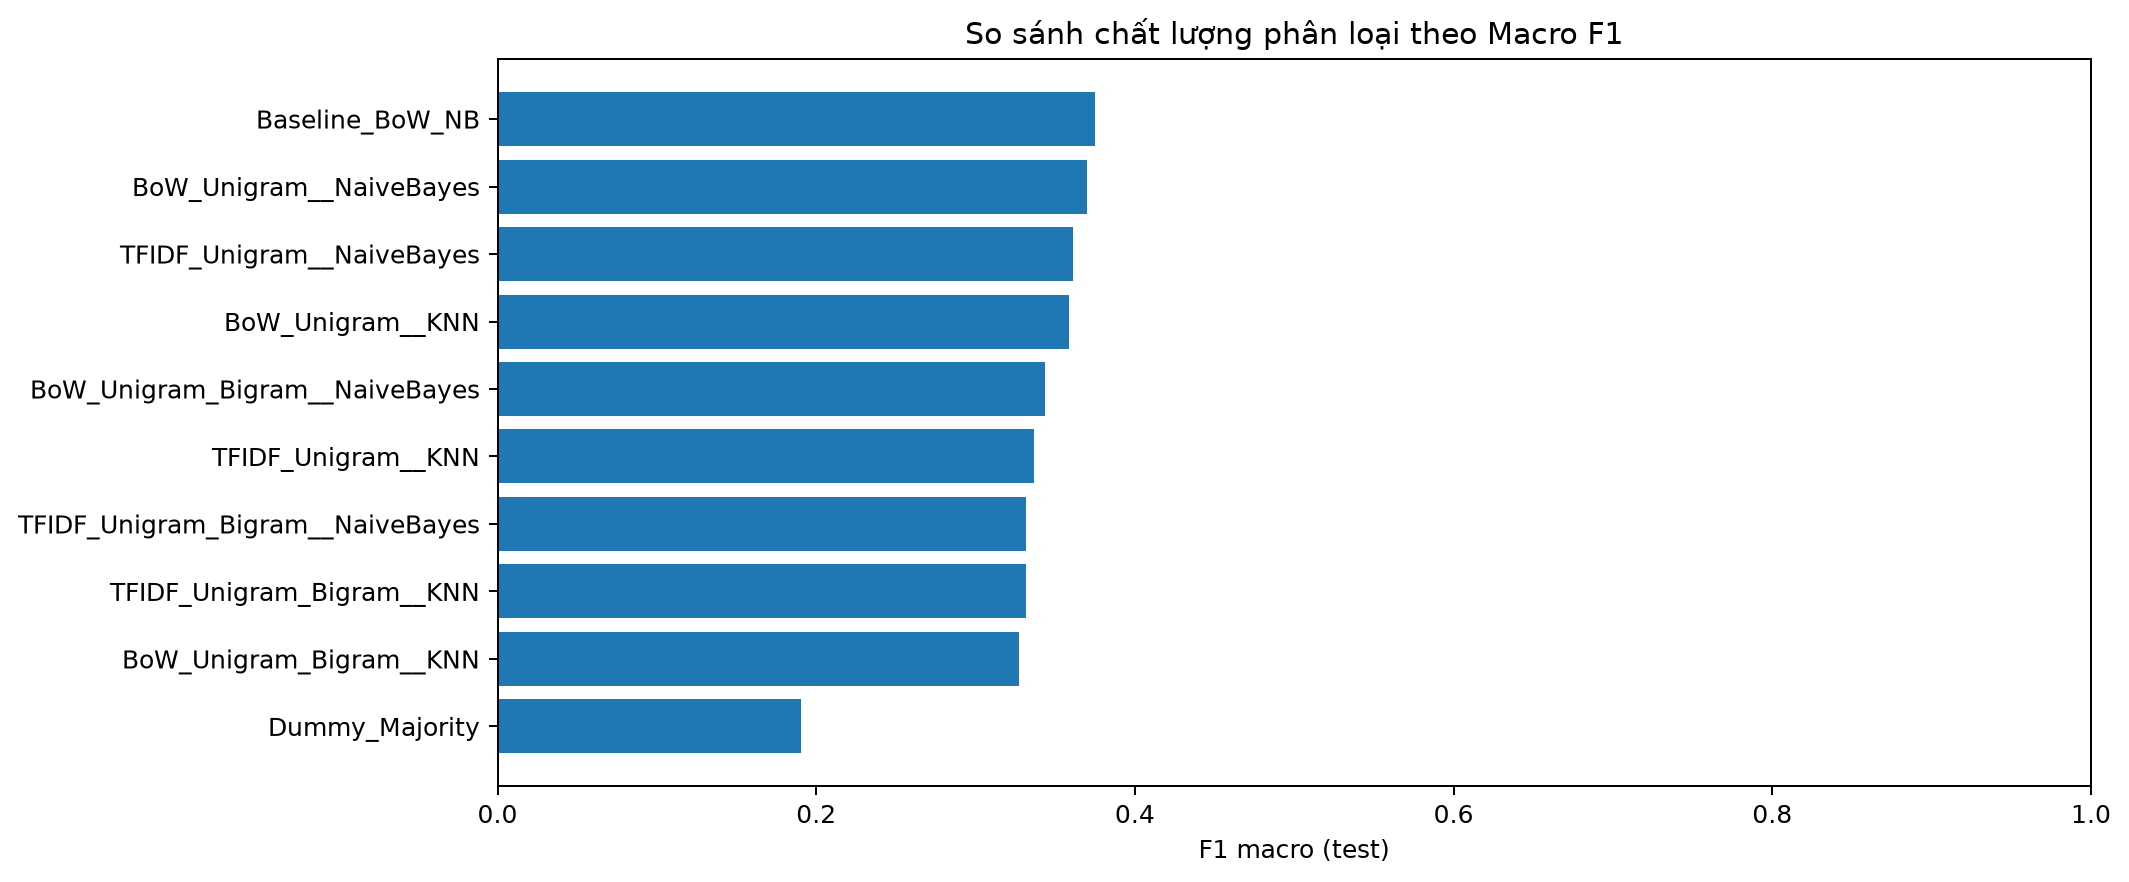
\includegraphics[
        width=0.92\textwidth
    ]{images/model_f1_comparison.png}
}{
    \fbox{
        \parbox[c][4cm][c]{0.85\textwidth}{
            \centering
            Chưa tải ảnh model\_f1\_comparison.png
        }
    }
}

\caption{So sánh Macro F1-score giữa các phương án}
\label{fig:ch4-so-sanh-f1}
\end{figure}

Hình~\ref{fig:ch4-so-sanh-f1} thể hiện sự
khác biệt về Macro F1-score giữa các cấu hình.

Các giá trị được lấy từ kết quả dự đoán trên
cùng một tập kiểm thử, do đó có thể sử dụng
để so sánh hiệu quả thực nghiệm của các
phương án trên bộ dữ liệu hiện tại.

\begin{figure}[H]
\centering

\IfFileExists{images/model_accuracy_comparison.png}{
    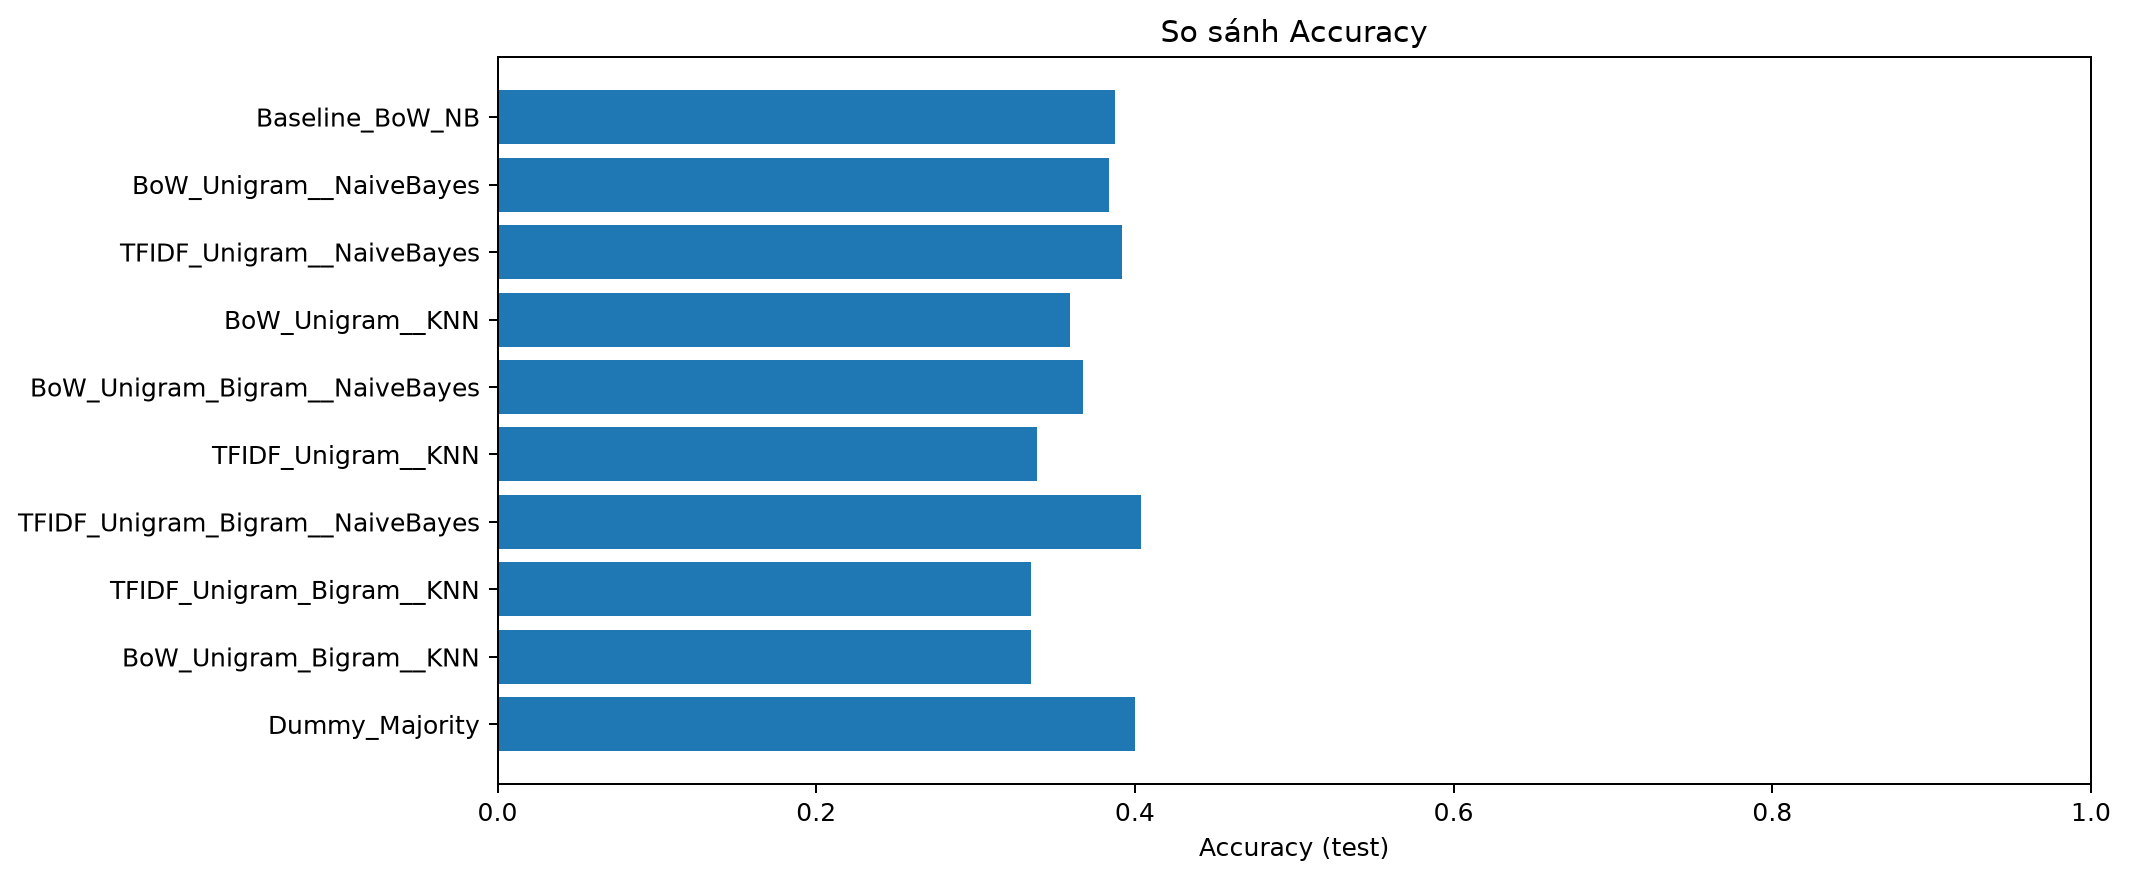
\includegraphics[
        width=0.92\textwidth
    ]{images/model_accuracy_comparison.png}
}{
    \fbox{
        \parbox[c][4cm][c]{0.85\textwidth}{
            \centering
            Chưa tải ảnh model\_accuracy\_comparison.png
        }
    }
}

\caption{So sánh Accuracy giữa các phương án}
\label{fig:ch4-so-sanh-accuracy}
\end{figure}

Khi đối chiếu Hình~\ref{fig:ch4-so-sanh-f1}
và Hình~\ref{fig:ch4-so-sanh-accuracy},
có thể nhận thấy thứ tự các phương án
không hoàn toàn giống nhau theo hai chỉ số.

Vì vậy, nhóm sử dụng kết hợp Accuracy,
Precision, Recall và Macro F1-score để
trình bày kết quả, thay vì chỉ dựa trên
một độ đo duy nhất.


\subsection{Kết quả của mô hình được lựa chọn bằng CV}

Mô hình TF-IDF Unigram kết hợp K-NN với
$k=5$ được lựa chọn dựa trên Macro F1-score
trung bình cao nhất trong quá trình
Cross-Validation.

Khi đánh giá trên tập test, mô hình đạt:

\begin{itemize}
    \item Accuracy: 0,3388.
    \item Precision Macro: 0,3431.
    \item Recall Macro: 0,3427.
    \item F1-score Macro: 0,3369.
\end{itemize}

Trong tổng số 245 phản hồi kiểm thử, mô hình
dự đoán đúng 83 phản hồi và dự đoán sai
162 phản hồi.

So với baseline, Macro F1-score của mô hình
được lựa chọn thấp hơn 0,0379 trên tập test.

Mặc dù mô hình có điểm CV cao nhất trong
các cấu hình thử nghiệm, kết quả trên tập
kiểm thử không cho thấy sự cải thiện so với
baseline.

Kết quả này được giữ nguyên để phục vụ
việc phân tích và thảo luận ở Chương 5.

% ============================================
% 4.5. THEO TỪNG NHÃN VÀ CONFUSION MATRIX
% ============================================

\section{Đánh giá theo từng lớp và ma trận nhầm lẫn}

\subsection{Kết quả phân loại theo từng lớp}

Để xem xét chi tiết khả năng nhận diện từng
nhãn cảm xúc, nhóm sử dụng Classification
Report của mô hình được lựa chọn bằng CV.

Kết quả được trình bày trong
Bảng~\ref{tab:ch4-ketqua-tung-lop}.

\begin{table}[H]
\centering
\caption{Kết quả phân loại theo từng lớp của TF-U + KNN}
\label{tab:ch4-ketqua-tung-lop}
\renewcommand{\arraystretch}{1.15}
\small

\begin{tabularx}{\textwidth}{|X|r|r|r|r|}
\hline
\textbf{Nhãn}
& \textbf{Precision}
& \textbf{Recall}
& \textbf{F1-score}
& \textbf{Số mẫu} \\
\hline

Negative
& 0,3069 & 0,4247 & 0,3563 & 73 \\
\hline

Neutral
& 0,3056 & 0,2973 & 0,3014 & 74 \\
\hline

Positive
& 0,4167 & 0,3061 & 0,3529 & 98 \\
\hline

\textbf{Macro avg}
& \textbf{0,3431}
& \textbf{0,3427}
& \textbf{0,3369}
& \textbf{245} \\
\hline

\end{tabularx}
\end{table}

Kết quả cho thấy nhãn Negative có Recall
cao nhất, đạt 0,4247.

Nhãn Neutral có Recall thấp nhất, đạt 0,2973,
trong khi nhãn Positive đạt Recall 0,3061.

Cả ba lớp đều có Recall dưới 0,5, cho thấy
mô hình chưa nhận diện chính xác được phần
lớn số phản hồi của từng lớp.

Sự khác biệt giữa các lớp được làm rõ hơn
thông qua ma trận nhầm lẫn ở mục tiếp theo.


\subsection{Ma trận nhầm lẫn}

Ma trận nhầm lẫn được sử dụng để thống kê
số lượng dự đoán đúng và sai giữa ba lớp
negative, neutral và positive.

Kết quả của mô hình TF-IDF Unigram kết hợp
K-NN được trình bày tại
Bảng~\ref{tab:ch4-confusion-matrix}.

\begin{table}[H]
\centering
\caption{Ma trận nhầm lẫn của TF-U + KNN}
\label{tab:ch4-confusion-matrix}
\renewcommand{\arraystretch}{1.15}
\small

\begin{tabular}{|l|r|r|r|}
\hline
\textbf{Nhãn thực tế}
& \multicolumn{3}{c|}{\textbf{Nhãn dự đoán}} \\
\cline{2-4}

& \textbf{Negative}
& \textbf{Neutral}
& \textbf{Positive} \\
\hline

Negative & 31 & 23 & 19 \\
\hline

Neutral & 29 & 22 & 23 \\
\hline

Positive & 41 & 27 & 30 \\
\hline

\end{tabular}
\end{table}

Trong ma trận, các giá trị trên đường chéo
chính tương ứng với số lượng mẫu được
dự đoán đúng.

Tổng số mẫu dự đoán đúng là:

\begin{equation}
31+22+30=83
\end{equation}

Do đó, Accuracy trên tập test được tính bằng:

\begin{equation}
\text{Accuracy}
=
\frac{83}{245}
\approx 0{,}3388
\end{equation}

Kết quả này phù hợp với chỉ số Accuracy do
chương trình đánh giá cung cấp.

Hình~\ref{fig:ch4-cm-knn} trực quan hóa
ma trận nhầm lẫn của mô hình được chọn.

\begin{figure}[H]
\centering

\IfFileExists{images/cm_TFIDF_Unigram__KNN.png}{
    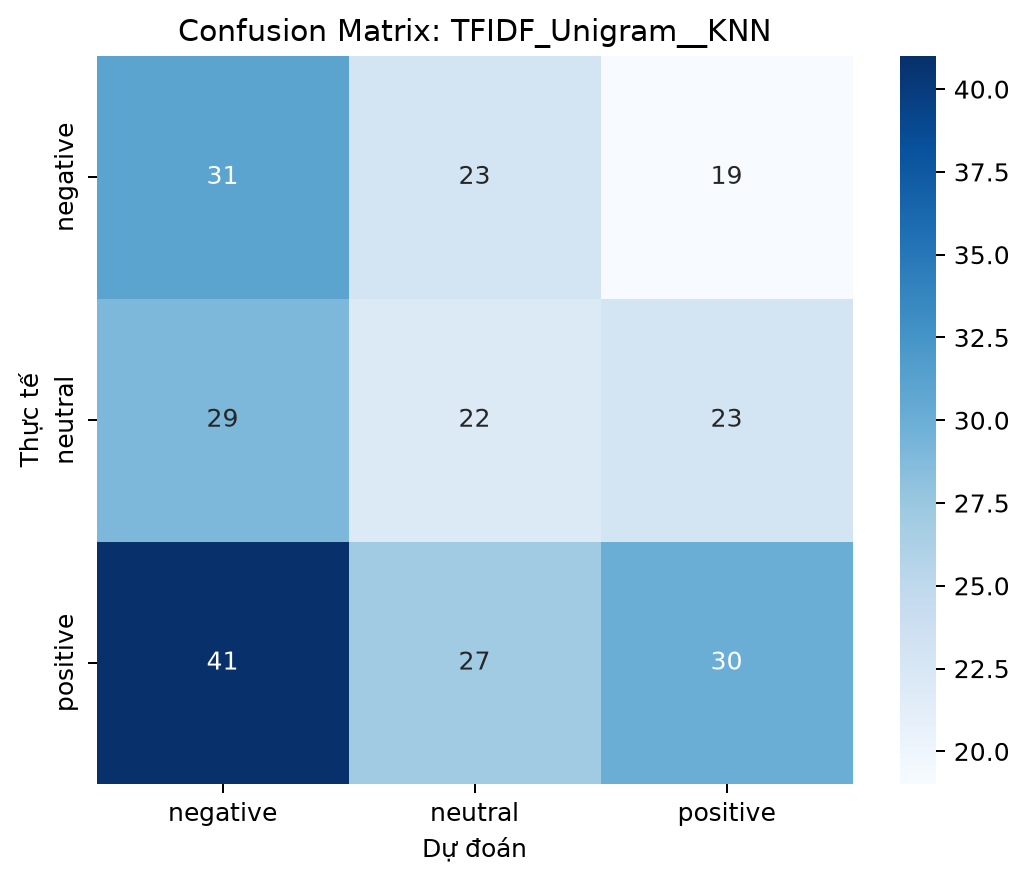
\includegraphics[
        width=0.76\textwidth
    ]{images/cm_TFIDF_Unigram__KNN.png}
}{
    \fbox{
        \parbox[c][4cm][c]{0.76\textwidth}{
            \centering
            Chưa tải ảnh Confusion Matrix
            của TF-IDF Unigram + KNN
        }
    }
}

\caption{Confusion Matrix của mô hình TF-U + KNN}
\label{fig:ch4-cm-knn}
\end{figure}

Từ ma trận nhầm lẫn, có thể thấy cặp nhãn
bị nhầm nhiều nhất là Positive được dự đoán
thành Negative, với 41 trường hợp.

Ngoài ra, có 29 phản hồi Neutral được dự
đoán thành Negative và 27 phản hồi Positive
được dự đoán thành Neutral.

Những số liệu trên cho thấy sai số xuất hiện
ở nhiều cặp nhãn khác nhau, không tập trung
vào một lớp duy nhất.

Để có thêm cơ sở so sánh, nhóm cũng trực
quan hóa ma trận nhầm lẫn của baseline.

\begin{figure}[H]
\centering

\IfFileExists{images/cm_Baseline_BoW_NB.png}{
    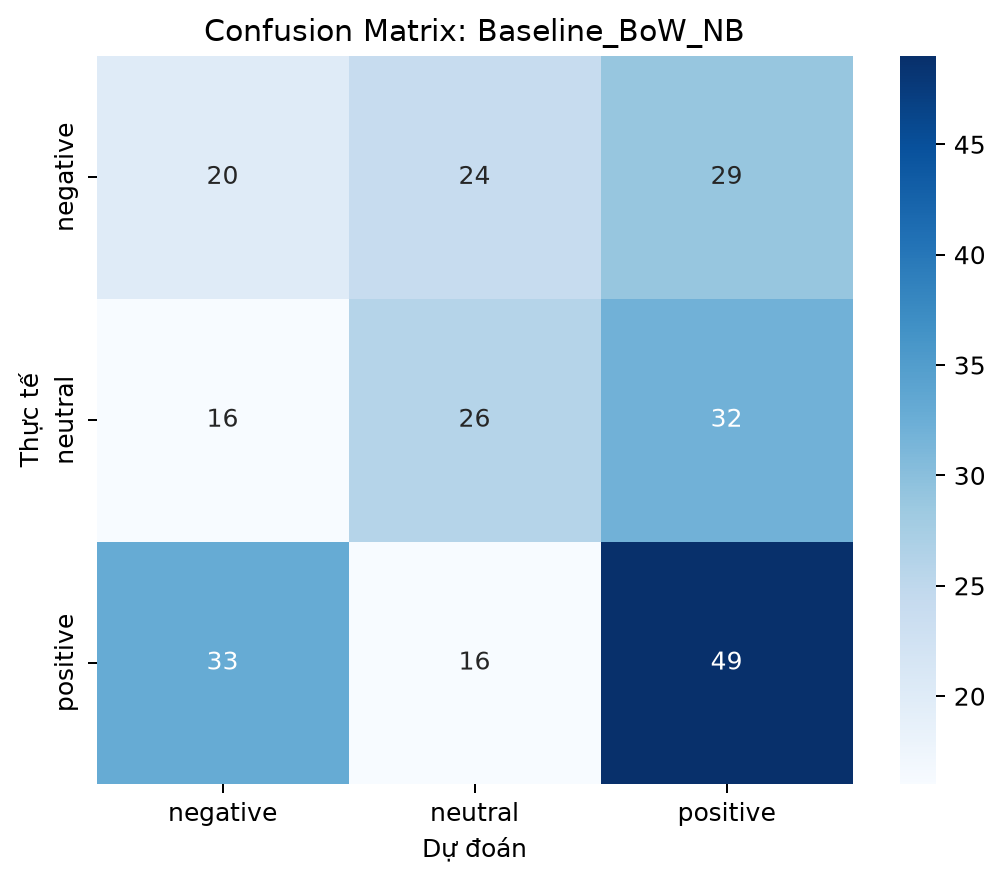
\includegraphics[
        width=0.76\textwidth
    ]{images/cm_Baseline_BoW_NB.png}
}{
    \fbox{
        \parbox[c][4cm][c]{0.76\textwidth}{
            \centering
            Chưa tải ảnh Confusion Matrix
            của baseline BoW + Naive Bayes
        }
    }
}

\caption{Confusion Matrix của mô hình baseline}
\label{fig:ch4-cm-baseline}
\end{figure}

Các ma trận nhầm lẫn được sử dụng làm căn cứ
để xác định các nhóm phản hồi mà mô hình
thường dự đoán sai.

Việc xem xét nội dung các phản hồi cụ thể
và những giả thuyết về nguyên nhân dự đoán
sai sẽ được thực hiện trong Chương 5.

% ============================================
% 4.6. TỔNG HỢP KẾT QUẢ
% ============================================

\section{Tổng hợp kết quả thực nghiệm}

Từ các thí nghiệm đã thực hiện, nhóm tổng
hợp được những kết quả chính như sau:

\begin{itemize}

    \item Nhóm đã triển khai hai thuật toán
    phân loại Multinomial Naive Bayes và K-NN,
    kết hợp với bốn cấu hình biểu diễn
    Bag-of-Words và TF-IDF.

    \item Có tổng cộng 24 lượt thử siêu tham số
    trên tập train bằng Stratified 3-Fold
    Cross-Validation.

    \item Cấu hình TF-IDF Unigram kết hợp K-NN
    với $k=5$ đạt Macro F1 trung bình cao nhất
    trên CV, bằng 0,3647.

    \item Trên tập test, cấu hình được lựa chọn
    đạt Accuracy 0,3388 và Macro F1-score
    0,3369.

    \item Baseline BoW Unigram kết hợp
    Multinomial Naive Bayes đạt Macro F1-score
    0,3748, cao hơn mô hình được chọn bằng CV
    trên tập kiểm thử hiện tại.

    \item Ma trận nhầm lẫn cho thấy mô hình
    được chọn dự đoán sai 162 trên tổng số
    245 phản hồi kiểm thử.

    \item Cặp nhãn bị nhầm nhiều nhất là
    Positive thành Negative, với 41 trường hợp.

\end{itemize}

Những kết quả trên cho thấy các phương pháp
học máy đã được triển khai và đánh giá theo
quy trình thực nghiệm thống nhất.

Tuy nhiên, hiệu quả phân loại trên tập
dữ liệu hiện tại còn hạn chế, đặc biệt
đối với việc nhận diện đồng thời cả ba
lớp cảm xúc.

Các chỉ số thu được cần được xem xét cùng
đặc điểm của bộ dữ liệu, phương pháp
biểu diễn đặc trưng và khả năng khái quát
hóa của mô hình.


% ============================================
% 4.7. TỔNG KẾT CHƯƠNG
% ============================================

\section{Tổng kết chương}

Chương 4 đã trình bày thiết lập thực nghiệm,
kết quả baseline, quá trình lựa chọn siêu
tham số bằng Cross-Validation và kết quả
đánh giá các mô hình trên tập kiểm thử.

Nhóm đã sử dụng Accuracy, Precision, Recall,
Macro F1-score và Confusion Matrix để đánh
giá hiệu quả của các phương án phân loại.

Kết quả cho thấy mô hình được lựa chọn bằng
Cross-Validation chưa đạt hiệu quả tốt hơn
baseline trên tập kiểm thử hiện tại.

Bên cạnh đó, ma trận nhầm lẫn và các chỉ
số theo từng lớp cho thấy mô hình vẫn gặp
khó khăn khi phân biệt các nhóm cảm xúc.

Trên cơ sở những kết quả này, Chương 5
sẽ tập trung thảo luận sự khác biệt giữa
các phương án, phân tích những trường hợp
dự đoán sai, xem xét hạn chế của dữ liệu
và đề xuất hướng cải tiến phù hợp.
